\documentclass{article}
\usepackage[utf8]{inputenc}
\usepackage[T1]{fontenc}
\usepackage{graphicx, float, svg} 
\usepackage{amsmath, amssymb, amsthm}
\usepackage[a4paper,margin=2.5cm]{geometry}

\title{Distance de Jaccard}
\author{Maysaloon BILAL \& Tristan GROULT}
\date{Mai 2025}

\begin{document}

\begin{figure}[t]
    \centering
    \begin{minipage}{0.3\textwidth}
        \centering
        
\includegraphics[width=1\textwidth]{logo_univ.png}
    \end{minipage}
    \hfill
    \begin{minipage}{0.3\textwidth}
        \centering
        
\includegraphics[width=1\textwidth]{ufr_logo.png}
    \end{minipage}
\end{figure}

\maketitle


\section{Introduction}

Ce projet consiste à développer un programme en langage C permettant de calculer la distance de Jaccard entre plusieurs fichiers texte, afin d’analyser leur similarité lexicale. La distance de Jaccard est une valeur comprise entre 0 et 1 : plus elle est proche de 0, plus les fichiers sont différents, et plus elle est proche de 1, plus ils sont similaires.

La distance de Jaccard entre deux ensembles $A$ et $B$ est définie par la formule :
\[
\text{Distance de Jaccard}(A, B) = 1 - \frac{|A \cap B|}{|A \cup B|}
\]

Le programme permet plusieurs personnalisations. Il est possible d’afficher un graphe indiquant à quels fichiers chaque mot appartient, ou d’activer un mode détaillé qui précise pour chaque mot les fichiers dans lesquels il apparaît. Une autre option permet également de définir une longueur maximale pour les mots analysés.

Pour gérer efficacement les mots extraits des fichiers, nous avons utilisé une table de hachage. Sa gestion — ajout, suppression, affichage du graphe, etc. — est implémentée dans le module \texttt{jaccard}. Ce projet s’appuie également sur deux autres modules : le module \texttt{word}, dédié à la création et la manipulation des mots, et le module \texttt{opt}, responsable du traitement des options en ligne de commande.

L’ensemble de ces composants est intégré et testé dans le fichier principal \texttt{main.c}, qui constitue le point d’entrée du programme.


\section{Méthodologie}

Dans cette section, nous expliquons les différentes étapes et approches utilisées pour implémenter le programme. Nous détaillerons la conception des modules, la gestion des fichiers et l’utilisation de la table de hachage.

\subsection{Module \texttt{word}}

Le module \texttt{word.c} sert à construire dynamiquement un mot caractère par caractère. Il est composé de 3 champs : 
\begin{itemize}
  \item Un champ \texttt{s} de type \texttt{char *} qui pointe vers un tableau de caractères qui stocke le mot lui-même.
  \item Un champ \texttt{length} de type \texttt{size\_t} qui représente la longueur du mot.
  \item Un champ \texttt{capacity} de type \texttt{size\_t} qui représente la capacité du tableau pointé par \texttt{s}
\end{itemize}

\begin{figure}[H]
    \centering
    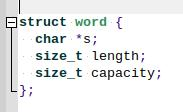
\includegraphics[width=0.4\textwidth]{word.jpg} 
    \caption{structure \texttt{word}}
    \label{fig:structure_word}
\end{figure}


\begin{itemize}
    \item \textbf{Initialisation d’un mot} : La fonction \texttt{word\_init()} permet de créer un nouveau mot avec une capacité initiale minimale définie par la constante \texttt{CAPACITY\_MIN}. Elle alloue dynamiquement de la mémoire pour la chaîne de caractères et initialise sa longueur à zéro.
    
    \item \textbf{Ajout d’un caractère au mot} : La fonction \texttt{word\_add()} ajoute un caractère à un mot. Si le mot atteint sa capacité maximale, la fonction double l'espace mémoire disponible avec \texttt{realloc()}, pour permettre l'ajout de nouveaux caractères. Cela permet au programme de gérer des mots de tailles variables sans perdre de données.
    
    \item \textbf{Réinitialisation du mot} : La fonction \texttt{word\_reinit()} permet de réinitialiser un mot, c'est-à-dire de remettre sa longueur à zéro et de vider la chaîne. Cela est utile lorsqu'un mot doit être réutilisé sans allouer de mémoire supplémentaire.
    
    \item \textbf{Accès à la chaîne de caractères} : La fonction \texttt{word\_get()} renvoie un pointeur vers la chaîne, tandis que \texttt{word\_get\_clean()} copie le mot dans dest, permettant ainsi de ne récupérer que le mot réel, sans les parties inutilisées de la mémoire allouée. Cela garantit que le mot est prêt à être utilisé sans risque de contenir des espaces "vides" dans la mémoire.
\end{itemize}


\begin{figure}[h]
    \centering
    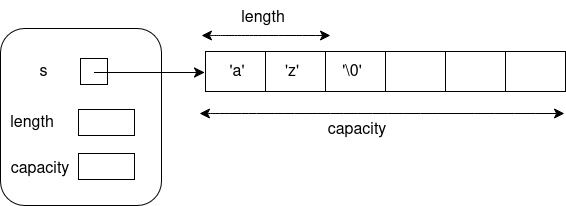
\includegraphics[width=0.7\textwidth]{word_schema.png} 
    \label{fig:structure_word_schema} 
\end{figure}

\subsection{Module \texttt{opt}}

Le module \texttt{opt} prend en charge le traitement des options fournies en ligne de commande.


\end{document}
